
%(BEGIN_QUESTION)
% Copyright 2003, Tony R. Kuphaldt, released under the Creative Commons Attribution License (v 1.0)
% This means you may do almost anything with this work of mine, so long as you give me proper credit

In each of the following circuits, the light bulb will energize when the pushbutton switch is actuated.  Assume that the supply voltage in each case is somewhere between 5 and 30 volts DC (with lamps and resistors appropriately sized):

$$\includegraphics[width=15.5cm]{i01005x01.eps}$$

However, not all of these circuits are properly designed.  Some of them will function perfectly, but others will function only once or twice before their transistors fail.  Identify the faulty circuits, and explain why they are flawed.

\underbar{file i01005}
%(END_QUESTION)





%(BEGIN_ANSWER)

Circuits 3, 5, and 6 are flawed, because the emitter-base junctions of their transistors are overpowered every time the switch closes.

\vskip 10pt

Hint: draw the respective paths of switch and lamp current for each circuit!

%(END_ANSWER)





%(BEGIN_NOTES)


%INDEX% Electronics review, transistor switch circuit (BJT)

%(END_NOTES)


